\subsection{Описание модели}

    Одна из вариаций модели Хасселя \cite{densityDependenceInSingleSpeciesPopulations} имеет следующую математическая запись:

    \begin{equation}
        \label{origin}
        x_{t+1} = \frac{\alpha x_t^2}{(\beta + x_t)^6}.
    \end{equation}

    В данной формуле \(x_t\) --- количество особей в поколении с номером \(t\). Параметр \(\alpha\) определяет скорость роста популяции, а параметр \(\beta\) определяет несущую способность окружающей среды.
    
    Для упрощения задачи рассмотрим частный случай. Зафиксируем параметр \(\alpha = 1\). Параметр \(\beta\) изменяется в диапазоне \([0; 0.6]\). Для нахождения равновесий требуется решить следующее уравнение:  

    \[x = \frac{\alpha x^2}{(\beta + x)^6}\]
    
    \[1 = \frac{\alpha x}{(\beta + x)^6}\]

    \begin{equation}
        \label{baseEquation}
        \alpha x = (\beta + x)^6
    \end{equation}

    Построим графики функций \(y = \alpha x\) и \(y = (\beta + x)^6\). 
        
    В зависимости от значений параметра \(\beta\) уравнение (\ref{baseEquation}) может иметь ноль (при \(\beta > 0.582355932\)), один (при \(\beta \approx 0.582355932\)) или два корня (при \(\beta < 0.582355932\)). На рисунках \ref{mainIntersect}, \ref{mainTouch} и \ref{mainOver} можно увидеть все возможные варианты. При \(\beta=0.582355932\) в модели наблюдается касательная бифуркации, сопровождающаяся появлением двух равновесий (см. рис. \ref{mainTouch}).

    \begin{figure}
        \centering
        \subfloat[\(\beta = 0.57\)]{
            \label{mainIntersect}
            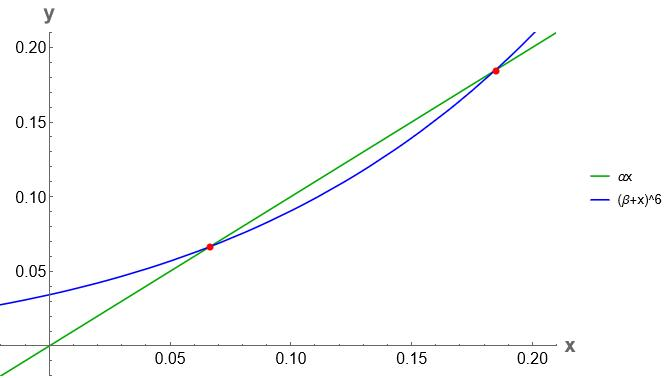
\includegraphics[width=0.5\textwidth]{deterministic/images/two_intersection.jpg}
        }
        \subfloat[\(\beta \approx 0.582355932\)]{
            \label{mainTouch}
            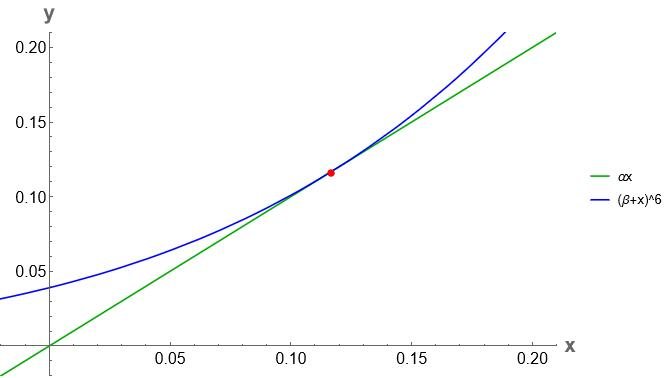
\includegraphics[width=0.5\textwidth]{deterministic/images/one_intersection.jpg}
        }

        \subfloat[\(\beta = 0.59\)]{
            \label{mainOver}
            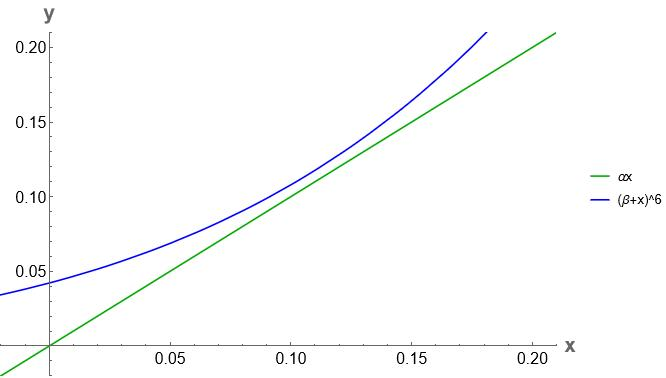
\includegraphics[width=0.5\textwidth]{deterministic/images/zero_intersection.jpg}
        } 
        % Было 0.75

        \captionsetup{justification=centering}
        \caption{Решения уравнения (\ref{baseEquation}) для разных значений параметра \(\beta\)}
    \end{figure}
